\chapter{Sistema PET}
Nella figura \ref{fig:PET_imaging_system} è rappresentato un sistema di imaging PET. Per rilevare i raggi gamma derivanti dal processo di annichilazione \textit{elettrone-positrone}, viene utilizzato un rilevatore a scintillazione, composto da uno scintillatore e un fotorilevatore. 
\begin{figure}[h]
	\centering
	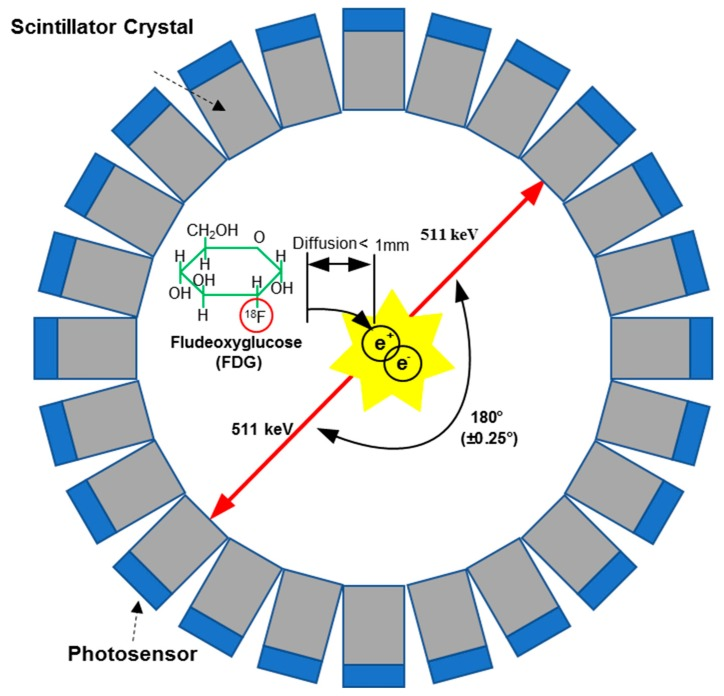
\includegraphics[width=0.5\linewidth]{./ImageFiles/PET_imaging_system}
	\caption{Principio di funzionamento di un sistema per tomografia ad emissione di positroni (PET). Un anello di sensori rilevano una coppia di raggi gamma con un'energia di \SI{511}{3\kilo\electronvolt} (frecce rosse) che derivano dalla annichilazione di un elettrone con un positrone emesso da un radiotracciante (FDG). Immagine tratta da Jiang W. et al \cite{Jiang2019}.}
	\label{fig:PET_imaging_system}
\end{figure}

\section{Scintillatori}
I cristalli scintillatori sono utilizzati per assorbire e convertire un raggio gamma ad alta energia in fotoni visibili a bassa energia, rilevati da opportuni sensori. Uno dei cristalli scintillatori più utilizzati è il \textit{Lutetium–(yttrium) oxyorthosilicate} (L(Y)SO) che garantisce una buona risoluzione di energia, alta luminosità in uscita e un tempo veloce di decadimento. Il processo di conversione di fotoni ad alta energia (raggi \textgamma) in luce visibile consiste in tre fasi \cite{RamseyDerek}:
\begin{itemize}
	\item un fotone incidente sul cristallo libera un elettrone (tramite effetto fotoelettrico o effetto Compton);
	\item quando l'elettrone attraversa il materiale, perde energia urtando ed eccitando altri elettroni;
	\item gli elettroni eccitati ritornano decadono al loro stato base, emettendo fotoni (sotto forma di impulsi di luce nel visibile).
\end{itemize}
Gli scintillatori utilizzati nei sistemi di acquisizione PET possono essere differenziati considerando quattro diverse proprietà \cite{Schmitz2013ThePO}:
\begin{itemize}
	\item stopping power;
	\item decay constant;
	\item energy resolution;
	\item light output.
\end{itemize}
Lo \textbf{stopping power} rappresenta l'inverso della distanza media percorsa dai fotoni prima di trasferire l'energia nel cristallo e dipende dalla densità e dal numero atomico effettivo del materiale. \`E preferibile che questo parametro sia alto (ossia poca distanza percorsa dai fotoni), in modo da avere più interazioni con i fotoni emessi dall'annichilazione \textit{elettrone-positrone}. La \textbf{decay constant}, invece, descrive la durata dell'impulso luminoso generato dal cristallo. \`E preferibile utilizzare cristalli con bassi valori di constante di decadimento in quanto permettono di rilevare un numero maggiore di impulsi a pari unità di tempo. Inoltre, è utile che il materiale abbia una buona risoluzione di energia (\textbf{energy resolution}), che descrive la capacità di distinguere raggi gamma con differenti energie. Infatti, nell'immagine \ref{fig:photo_peak} è mostrato lo spettro di distribuzione di energia, costruito misurando il numero di eventi rilevati con una certa ampiezza in funzione dell'energia depositata sul cristallo.
\begin{figure}[h]
	\centering
	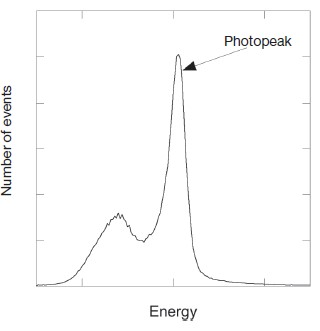
\includegraphics[width=0.4\linewidth]{./ImageFiles/Photo peak.jpg}
	\caption{Esempio di uno spettro di energia, definito come il numero di eventi misurati con una certa ampiezza in funzione della energia depositata sul cristallo. Immagine tratta da Bailey D et al. \cite{Bailey2014}.}
	\label{fig:photo_peak}
\end{figure}
Questa distribuzione è influenzata dalle caratteristiche del tracciatore radioattivo utilizzato e dal materiale con cui è realizzato il rilevatore. Tuttavia, è possibile sempre notare un picco marcato (denominato \textit{photopeak}), causato dall'assorbimento fotoelettrico, dove tutta l'energia del fotone è trasmessa all'elettrone. L'altra regione in cui l'energia si distribuisce è invece causata dall'effetto Compton, dove gli elettroni acquistano diversi valori di energia in base all'angolo di scattering. L'obiettivo delle tecniche di imaging della medicina nucleare è quello di riuscire a distinguere i raggi gamma che non hanno avuto interazioni con altri tessuti, che ne hanno provocato una deviazione. I fotoni di interesse sono proprio quelli i cui raggi \textgamma hanno energia pari al \textit{photopeak} e che, non essendo stati soggetti a fenomeni di scattering, permettono di risalire in modo accurato alla posizione del radionuclide. Tipicamente, il \textit{photopeak} si presenta in un valore di energie nell'intervallo \numrange[range-phrase=--]{440}{650}\,\unit{\kilo\electronvolt}. Infine, il parametro \textbf{light output} definisce il numero di fotoni emessi durante la scintillazione prodotti da ogni fotone incidente. Il valore di questo parametro dovrebbe essere il più alto possibile per garantire la massima risoluzione spaziale e di energia.

\noindent
Il confronto tra alcune caratteristiche di diversi scintillatori utilizzati negli scanner PET sono riportate nella tabella \ref{tab:scintillator_properties}.

\begin{table}[tbh]
	\centering
	\begin{tabular}{l|ccc}
		\hline
		\textbf{Cristallo} & NaI & BGO & LSO (LYSO) \\ \hline
		\textbf{Stopping power} ($\unit{\centi\meter}^{-1}$) & 0.34 & 0.92 & 0.87  \\ \hline
		\textbf{Decay constant} (\unit{\nano\second}) & 230 & 300 & 40 \\ \hline
		\textbf{Light output} (\%NaI:TI) & 100 & 15 & 75 \\ \hline
	\end{tabular}
	\caption{Proprietà dei materiali scinitallori utilizzati negli scanner PET. Dati tratti da \cite{RamseyDerek}.}
	\label{tab:scintillator_properties}
\end{table}

\section{Fotorilevatori}
Per convertire il segnale luminoso in segnale elettrico si utilizzano dei fotorilevatori, come ad esempio i \textit{Photomultiplier Tubes} (PMTs), Avalanche Photodiodes (ADPs) e i Silicon Photomultipliers (SiPMs). Nella figura \ref{fig:photodetectors_performance} sono presentanti in modo riassuntivo le caratteristiche dei diversi fotorilevatori utilizzati.
\begin{figure}[tbh]
	\centering
	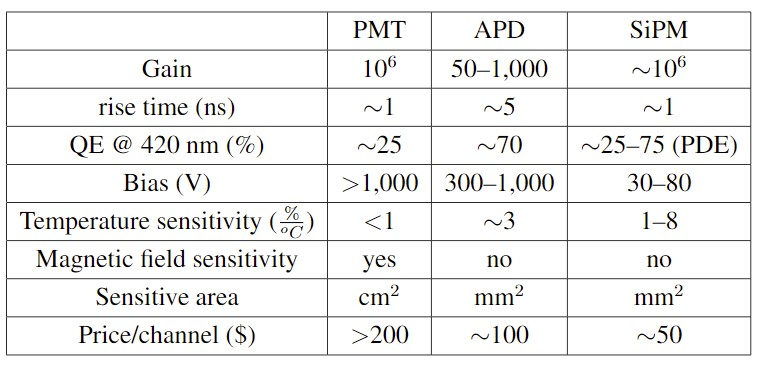
\includegraphics[width=0.7\linewidth]{./ImageFiles/table_pet_detectors_properties.jpg}
	\caption{Confronto delle caratteristiche di diversi rilevatori utilizzati nella tomografia a emissione di positroni. Immagine tratta da Spanoudaki V. e Levin C.\cite{Spanoudaki2010}}. 
	\label{fig:photodetectors_performance}
\end{figure}
Si creano quindi dei moduli (\Fig\ref{fig:photodetectors}) costituiti da uno scintillatore montato su un fotorilevatore.
\begin{figure}[tbh]
	\centering
	a)
	\begin{minipage}{.45\textwidth}
		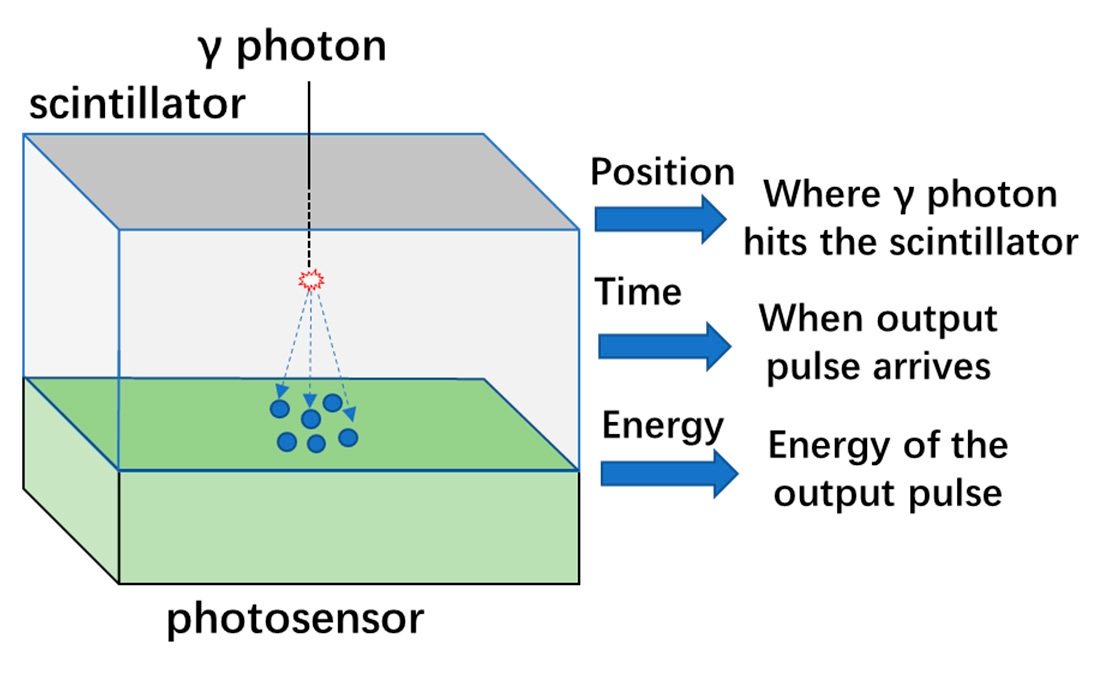
\includegraphics[width=\linewidth]{./ImageFiles/PET_detectors.jpg}
	\end{minipage}
	b)
	\begin{minipage}{.45\textwidth}
		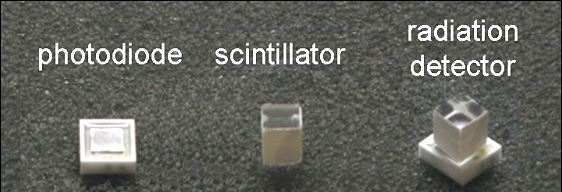
\includegraphics[width=\linewidth]{./ImageFiles/PET_detectors_real.jpg}
	\end{minipage}
	\caption{Struttura di un sensore PET. Immagini tratte da \cite{Jiang2019} e da \cite{Spanoudaki2010}.}
	\label{fig:photodetectors}
\end{figure}
Questi \textit{detectors} modulari sono poi uniti per formare un anello al centro del quale rilevare i raggi gamma (\Fig\ref{fig:PET_imaging_system}). I rilevatori utilizzati per la PET devono permettere di ricavare tre tipi di informazioni:
\begin{itemize}
	\item la posizione di dove il raggio gamma impatta lo scintillatore;
	\item il tempo in cui si verifica l'impulso luminoso;
	\item l'energia dell'impulso luminoso generato.
\end{itemize}
Di seguito si analizzano alcuni fotorivelatori utilizzati nei sistemi PET.

\subsection{Photomultiplier Tubes}
Nella figura \ref{fig:ptm} è mostrato lo schema della struttura di un fotomoltiplicatore PMT (\textit{Photomultiplier Tube}).
\begin{figure}[tbh]
	\centering
	a)
	\begin{minipage}{.70\textwidth}
		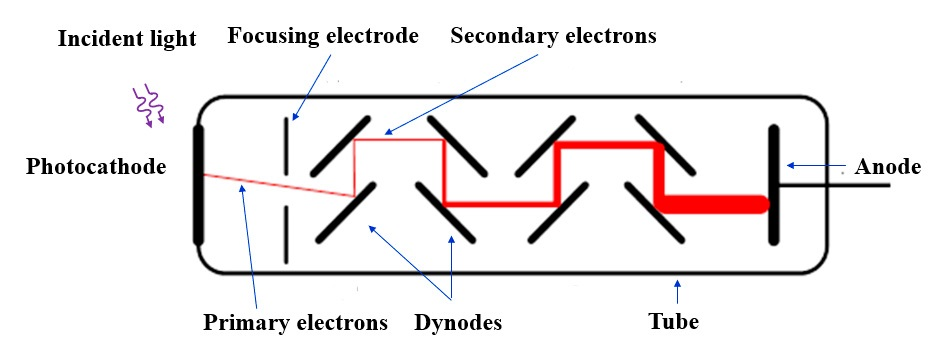
\includegraphics[width=\linewidth]{./ImageFiles/ptm.jpg}
	\end{minipage}

	b)
	\begin{minipage}{.70\textwidth}
		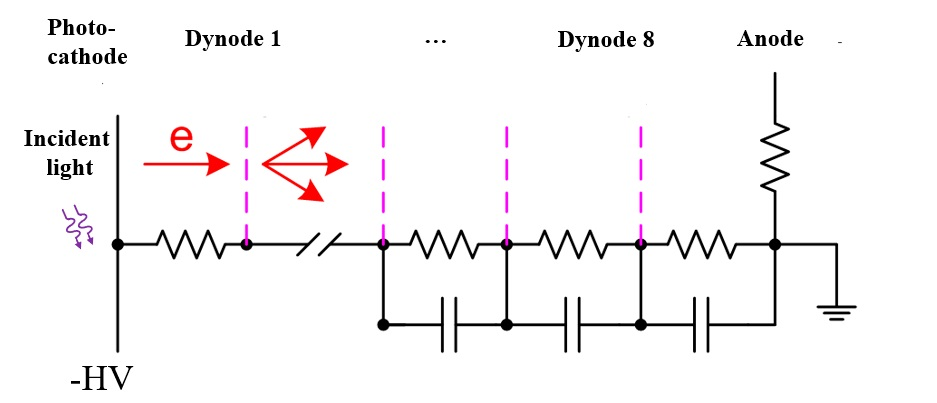
\includegraphics[width=\linewidth]{./ImageFiles/ptm_schema.jpg}
	\end{minipage}
	\caption{Principio di funzionamento di un \textit{photomultiplier tube} (PTM): a) struttura semplificata; b) schema semplificato del circuito di polarizzazione ad alta tensione. Immagine tratta da Jiang et al. \cite{Jiang2019}.}
	\label{fig:ptm}
\end{figure}
Esso è composto da un \textit{fotocatodo}, una serie di elettrodi chiamati \textit{dinodi} e un \textit{anodo}, inseriti in un tubo di vetro al cui interno è stato praticato il vuoto. Ai differenti dinodo è applicata una tensione crescente che permette di aumentare progressivamente il campo elettrico all'interno del tubo. I fotoni incidenti sul fotocatodo (ricoperto da un materiale che favorisce l'effetto fotoelettrico) generano degli elettroni (denominati \textit{fotoelettroni}) che vengono focalizzati da un elettrodo verso il primo dinodo. A causa del forte campo elettrico generato dalla differenza di potenziale tra il primo dinodo e il fotocadoto, gli elettroni primari aumentano la propria energia cinetica. Quando un elettrone fotogenerato colpisce il primo dinodo provoca l'emissione secondaria di diversi elettroni con minore energia. La struttura è realizzata in modo che ciascun elettrone secondario venga accelerato verso il dinodo successivo e provochi quindi l'emissione di ulteriori elettroni secondari. Si instaura così un fenomeno a cascata per cui un singolo elettrone fotogenerato genera un numero di elettroni pari a 
\begin{equation}
	G = f^n,
\end{equation}
dove $f$ è il fattore di emissione di elettroni secondari di ogni dinodo e n è il numero di dinodi. Valori tipici delle tensioni di alimentazioni sono  compresi nell'intervallo di \numrange[range-phrase=--]{1000}{2000}\,\unit{\kilo\volt} e il guadagno $G$ raggiunto è di circa di $G=10^6$. Per determinare la posizione dell'interazione \textit{fotone-cristallo scintillatore}, è possibile utilizzare una struttura definita a \textit{block detector} (\Fig\ref{fig:block_detector}).
\begin{figure}[tbh]
	\centering
	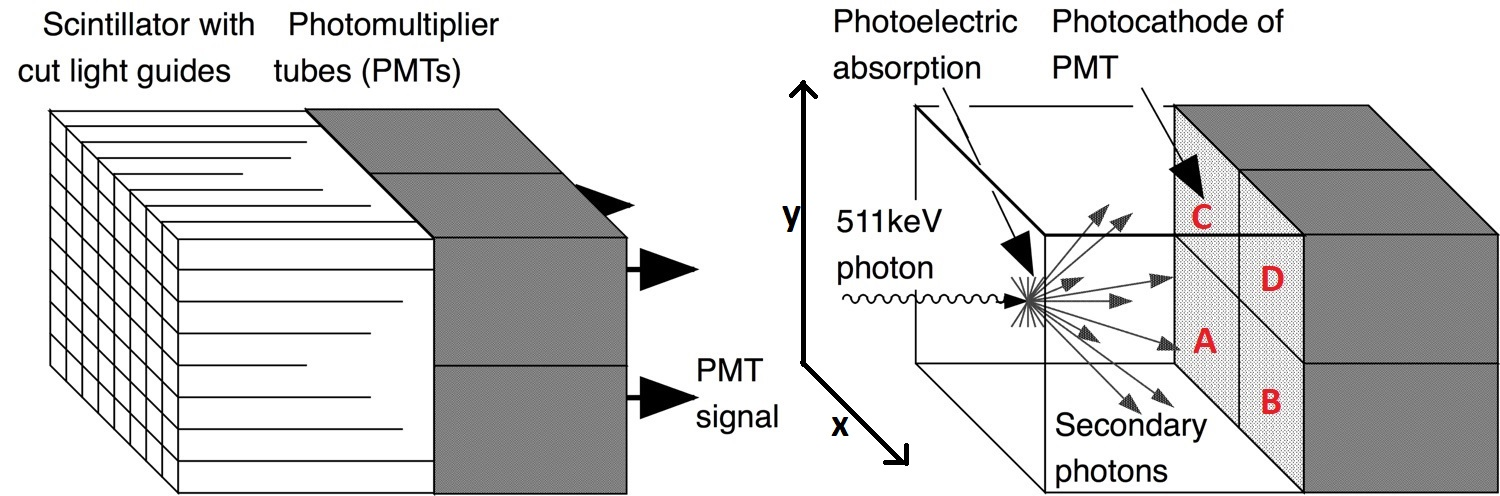
\includegraphics[width=0.8\linewidth]{./ImageFiles/block_detector.jpg}
	\caption{Schema della struttura di un \textit{block detector} con piccoli cristalli scintillatori raggruppati in blocchi accoppiati a quattro PMT. Immagine tratta da Schmitz et al. \cite{Schmitz2013ThePO}}. 
	\label{fig:block_detector}
\end{figure}
Viene ricavato da un cristallo una matrice di blocchi scitillatori (di dimensioni di qualche millimetro), suddivisi da un materiale riflettente. Gli impulsi luminosi emessi vengono letti da 4 differenti PMT (\Fig\ref{fig:block_detector_cube}).
\begin{figure}[tbh]
	\centering
	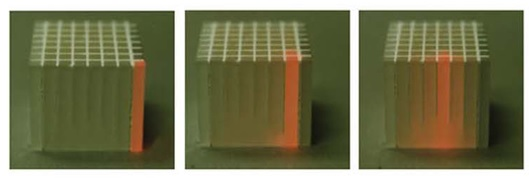
\includegraphics[width=0.6\linewidth]{./ImageFiles/block_detector_lightoncube.jpg}
	\caption{Distribuzione della luce in un cristallo scintillatore suddiviso in una matrice di cristalli. Immagine tratta da Terry Jones e David Townsend \cite{Jones2017}}. 
	\label{fig:block_detector_cube}
\end{figure}
Confrontando le intensità rilevate dai quattro PMT con dei valori pre-calcolati, è possibile ricavare la posizione del fotone incidente sul piano tramite le seguenti equazioni \cite{RamseyDerek} (logica di Anger):
\begin{equation}
	\begin{split}
		R_X&=\frac{A+B}{A+B+C+D} \\
		R_Y&=\frac{A+C}{A+B+C+D}, \\
	\end{split}
\end{equation}
dove $A,B,C,D$ rappresentano la frazione di luce misurata dai quattro PMT.

Idealmente, se nessun fotone viene assorbito dal fotocatodo (ossia se il sensore viene tenuto al buio), non ci sarà nessun segnale all'anodo del PMT. Tuttavia, statisticamente c'è una probabilità non nulla che degli elettroni vengano emessi dal fotocadoto e dai dinodi per effetto termoionico, generando un impulso. Ciò determina il parametro di\textit{dark count rate} (DCR) del PMT (tipicamente pari a 10 impulsi al secondo). \todo{inserire pag 8 sesnor for positron TTR e TTs}
Un altro parametro di interesse per descrivere un PMT è la \textit{Photon detection efficiency} (PDE) che descrive la probabilità di emissione di un elettrone fotogenerato per ogni fotone incidente, che dipende dalla \textit{quantum efficiency} (QE) del materiale che ricopre il fotocatodo e dalla \textit{collection efficiency} (CE), ossia il rapporto tra il numero di elettroni che giungono al primo dinodo e quelli generati dal fotocatodo \cite{Hai2018}. La QE di un PMT è tipicamente pari al \SI{25}{\percent}, ma la PDE assume un valore minore a causa della CE, dal momento che non tutti gli elettroni fotogenerati generano un impulso luminoso.

Sebbene i PMT abbiano un alto guadagno, alta risoluzione nel tempo, basso \textit{noise} e una QE accettabile, presentano alcuni svantaggi. Infatti, sono molto fragili e sensibili a vibrazioni meccani e disturbi elettromagnetici e necessitano di alte tensioni di alimentazione. Per questo motivo sono state sviluppate soluzioni a stato solido come gli ADP e i SiPM.

\newpage
\subsection{Avalanche Photodiodes}
Gli \textit{avalanche photodiodes} (APDs) sono diodi che strutturalmente sono simili ai p-n e p-i-n fotodiodi ma presentano un meccanismo di guadagno determinato da un eventi "a valanga". Essi sono fortemente polarizzati inversamente (tipicamente \numrange[range-phrase=--]{100}{200}\,\unit{\volt}), generando un forte campo magnetico nella zona di svuotamento. In questo modo, quando un elettrone viene generato da un fotone incidente (effetto fotoelettrico) nella zona di svuotamento subisce una accelerazione tale che, all'impatto con gli atomi del reticolo del substrato circostante, genera una coppia elettrone-lacuna (\Fig\ref{fig:apd}). 
\begin{figure}[tbh]
	\centering
	a)
	\begin{minipage}{.45\textwidth}
		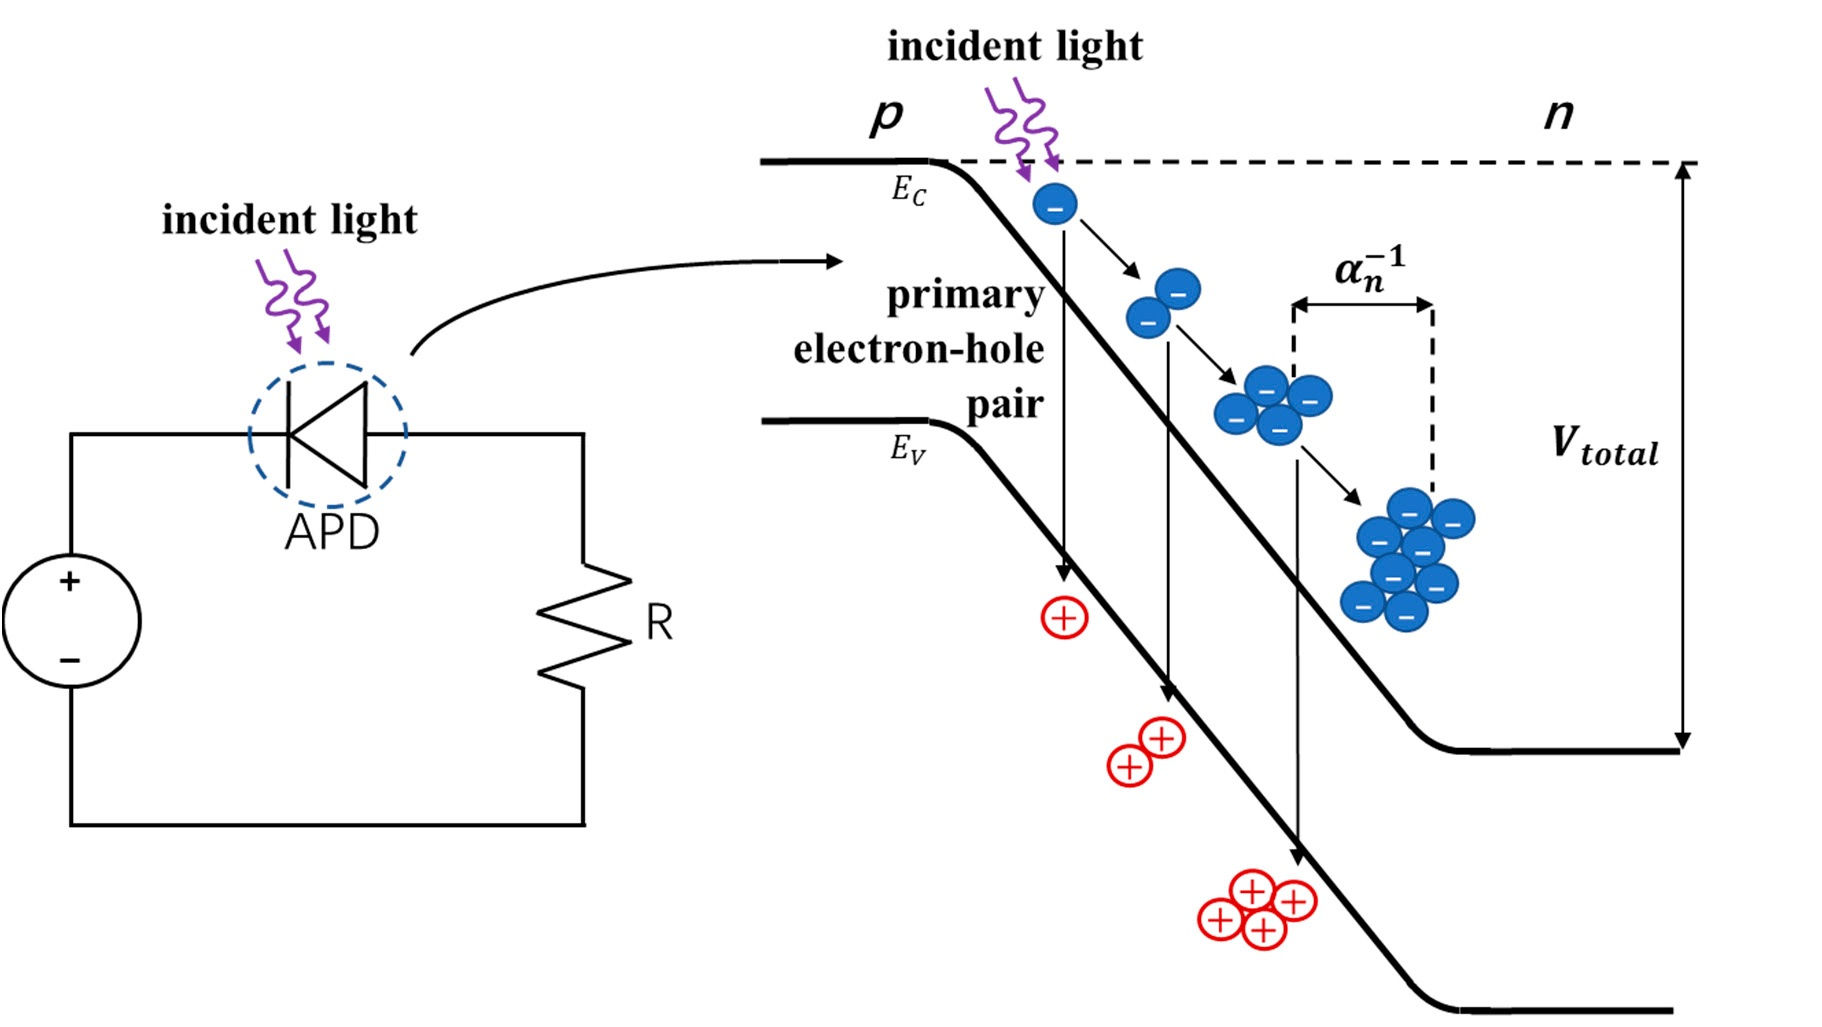
\includegraphics[width=\linewidth]{./ImageFiles/APD.jpg}
	\end{minipage}
	b)
	\begin{minipage}{.45\textwidth}
		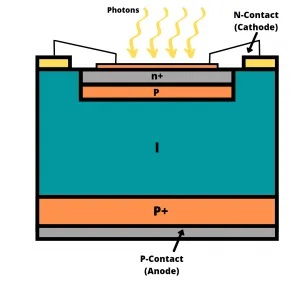
\includegraphics[width=\linewidth]{./ImageFiles/apd_2D.jpg}
	\end{minipage}
	c)
	\begin{minipage}{.45\textwidth}
		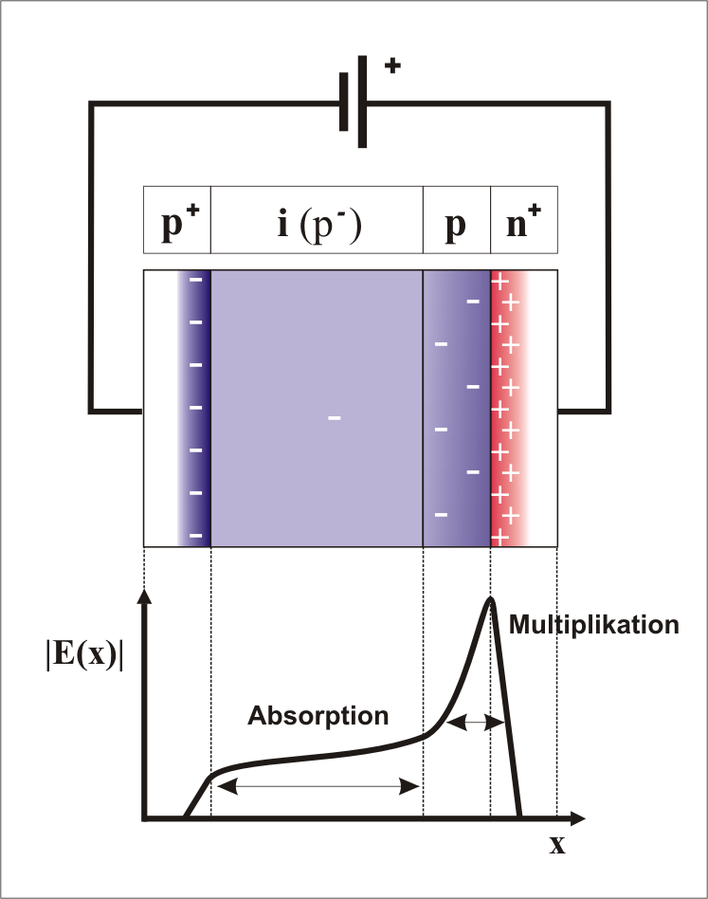
\includegraphics[width=\linewidth]{./ImageFiles/APD2_German.png}
	\end{minipage}
	d)
	\begin{minipage}{.45\textwidth}
		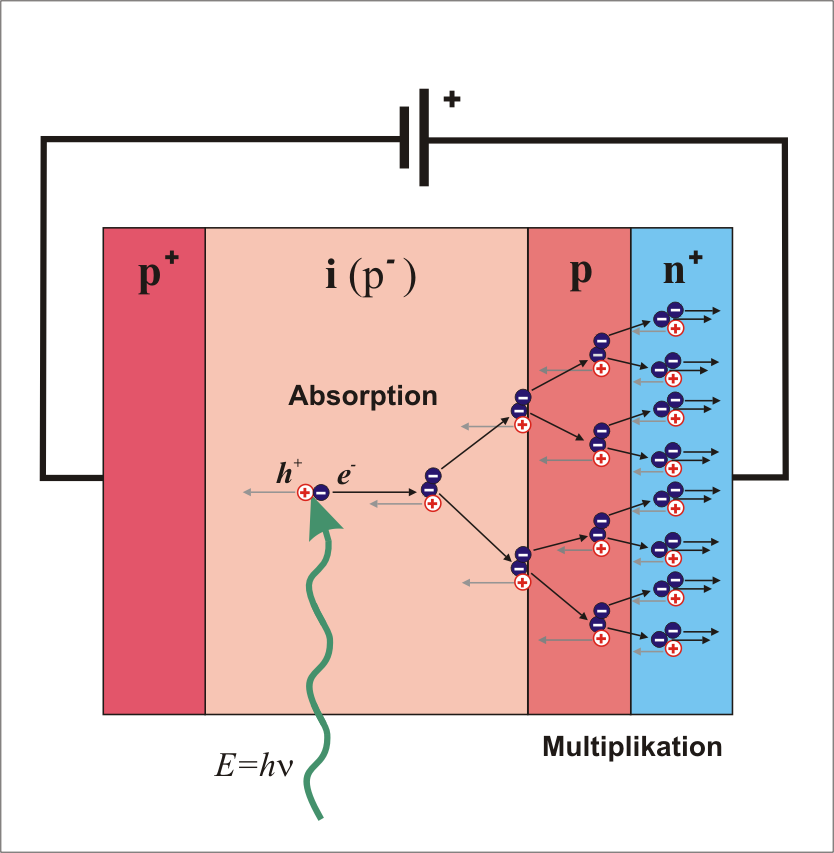
\includegraphics[width=\linewidth]{./ImageFiles/APD3_German.png}
	\end{minipage}
	\caption{Effetto a valanga e struttura di un diodo APD. Nella figura a), $\alpha_n^{-1}$ è la distanza media tra ogni evento di moltiplicazione e $V_{TOT}$ è la tensione di polarizzazione (sommata al potenziale di built-in). Immagine tratta da Wei Jiang et al. \cite{Jiang2019} e \cite{ApdImage}.} 
	\label{fig:apd}
\end{figure}
Il fenomeno si definisce \textit{ionizzazione per impatto} e si ripete a cascata per ogni elettrone generato. Il risultato è un incremento della corrente misurabile. Il guadagno di moltiplicazione $M$ è determinato dal coefficiente \textalpha (coefficiente di ionizzazione per impatto) per i portatori primari e indica il numero di coppie elettrone-lacuna generate per unità di lunghezza \cite{Jiang2019} dal portatore.
L'effetto a valanga è un evento stocastico in quanto non è detto che tutti i portatori fotogenerati o iniettati portano allo stesso numero di eventi di moltiplicazione. Questa caratteristica è misurata dal parametro $F$ definito \textit{excess noise factor} che dipende dal rapporto tra i coefficienti di ionizzazione delle lacune e degli elettroni del materiale usato. Infatti, si definisce $k=\alpha_p / \alpha_n$. Valori tipici di $k$ sono circa di 0.02 per il silicio e 0.5 per APD con Ge. Per minimizzare il rumore, si tenderà a minimizzare il valore di $k$. Per questa ragione, la maggior parte dei diodi APD in commercio sono composti dal silicio. Più precisamente, la relazione tra $F$ e $k$ è descritta dall'equazione \cite{HAMAMATSU2021}\cite{Hossain2019}:
\begin{equation}
	F=Mk+(2-\frac{1}{M})(1-k)
\end{equation}
Tuttavia, il guadagno $M$ è influenzato da diversi fattori, quali la temperatura, la lunghezza d'onda della luce incidente e dalla tensione inversa applicata \ref{fig:apd_gain}. Quindi, anche $F$ dipenderà da questi fattori. 
\begin{figure}[tbh]
	\centering
	a)
	\begin{minipage}{.45\textwidth}
		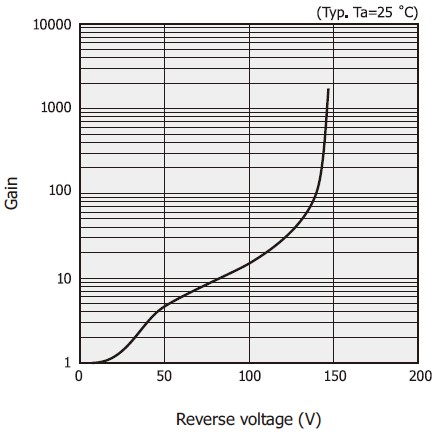
\includegraphics[width=\linewidth]{./ImageFiles/apd_gain_rv.jpg}
	\end{minipage}
	b)
	\begin{minipage}{.45\textwidth}
		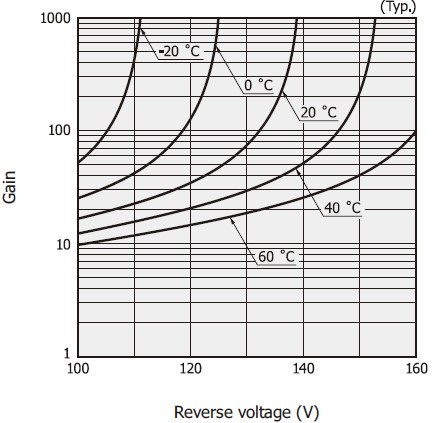
\includegraphics[width=\linewidth]{./ImageFiles/apd_gain_temp.jpg}
	\end{minipage}
	c)
	\begin{minipage}{.45\textwidth}
		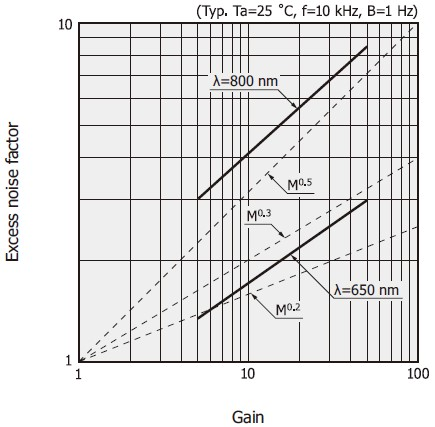
\includegraphics[width=\linewidth]{./ImageFiles/apd_wave1.jpg}
	\end{minipage}
	d)
	\begin{minipage}{.45\textwidth}
		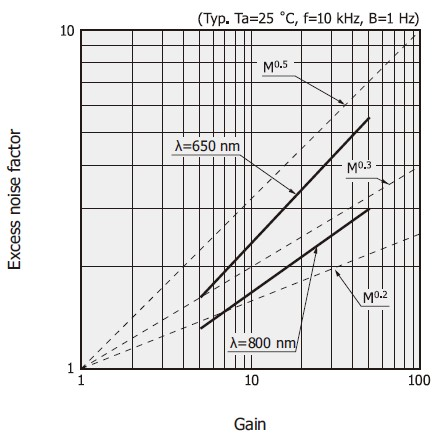
\includegraphics[width=\linewidth]{./ImageFiles/apd_wave2.jpg}
	\end{minipage}
	\caption{Esempi di dipendenza del guadagno $M$ dalla tensione di polarizzazione inversa a), dalla temperatura b) e dipendenza dell'\textit{excess noise factor} dalla lunghezza d'onda della luce incidente c) e d). Immagine tratta da HAMAMATSU PHOTONICS K.K \cite{HAMAMATSU2021}.}
	\label{fig:apd_gain}
\end{figure}
Le performance dei diodi a valanga sono anche determinati dalla \textit{spectral response}, \textit{quantum efficiency} (QE) e \textit{dark current}. La \textit{spectral response} descrive la corrente (A) generata per unita di potenza (W) della luce incidente per diverse lunghezze d'onda \cite{Jiang2019}. Anche la \textit{quantum efficiency} dipende dalla lunghezza d'onda e definisce la percentuale di fotoni che raggiunge la zona di svuotamento e genera un evento a valanga. Sebbene i APD abbiano un guadagno interno tipicamente minore (che può variare dai \numrange[range-phrase=--]{25}{1000}) dei PTM, stanno avendo molto successo negli ultimi anni, grazie al minor costo, alle ridotte dimensioni e alla insensibilità ai campi magnetici (caratteristica usata nei sistemi ibridi PET/MRI).

\clearpage
\subsection{Silicon Photomultipliers}
Per migliorare ulteriormente le performance dei fotorilevatori, sono stati introdotti i Silicon Photomultiplier (SiPM). Questi dispositivi sono costituiti da una matrice di microscopici pixel, connessi in parallelo, costituiti da APD che operano nella cosiddetta modalità Geiger (denominati anche SPAD). Un Single Photon Avalanche Diode (SPAD) è costituito da una giunzione p-n polarizzata inversamente con una tensione $V_{EX}$ maggiore della tensione di breakdown $V_{BR}$, operando nella modalità definita Geiger \cite{Jiang2019}. Il valore del campo elettrico nella regione di svuotamento è tale che la corrente generata a causa di un singolo fotone assume valori molto alti, producendo un impulso di corrente. Inoltre, la corrente generata dalla valanga continuerà a fluire fino a quando il campo elettrico non si ridurrà al di sotto della soglia di \textit{breakdown} e sarà quindi possibile rilevare un successivo fotone \cite{Palubiak2011}. Per fermare l'evento a valanga, si utilizza un circuito \textit{quenching}, che nella sua realizzazione più semplice è costituito da un resistore di valore elevato in serie al fotodiodo. Nella figura \ref{fig:spad_VI}a) è rappresentata la giunzione p-n polarizzata inversamente e la resistenza R\sub{Q} di quenching. Nella figura \ref{fig:spad_VI}b) è descritta la caratteristica V-I di un diodo fotorivelatore a singolo fotone. Inizialmente, il diodo è spento (1), ossia attraverso il diodo scorre solo la corrente inversa. Successivamente, quando un elettrone entra nella zona di svuotamento, il fenomeno a valanga genera una corrente di valore elevato (2). A causa della presenza della resistenza R\sub{Q} (di valore elevato), la corrente generata determina una caduta di potenziale che porta la tensione ai capi del diodo al di sotto della tensione di brakdown (3). L'evento a valanga quindi si interrompe e la tensione ai capi del diodo si riporta alla tensione di polarizzazione iniziale dopo un tempo definito di \textit{hold off}, che dipende la costante di tempo $\tau_{Hoff}=R_QC_{SPAD}$, dove $C_SPAD$ è la capacità parassita associata al diodo.
\begin{figure}[tbh]
	\centering
	a)
	\begin{minipage}{.45\textwidth}
		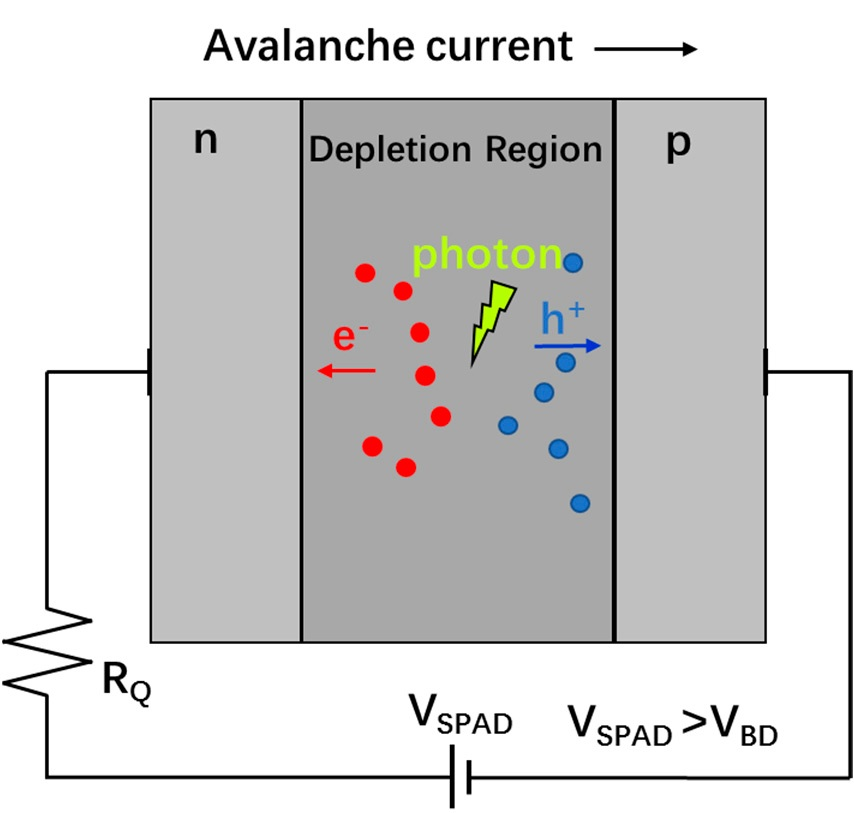
\includegraphics[width=0.8\linewidth]{./ImageFiles/spad_scheme.png}
	\end{minipage}
	b)
	\begin{minipage}{.45\textwidth}
		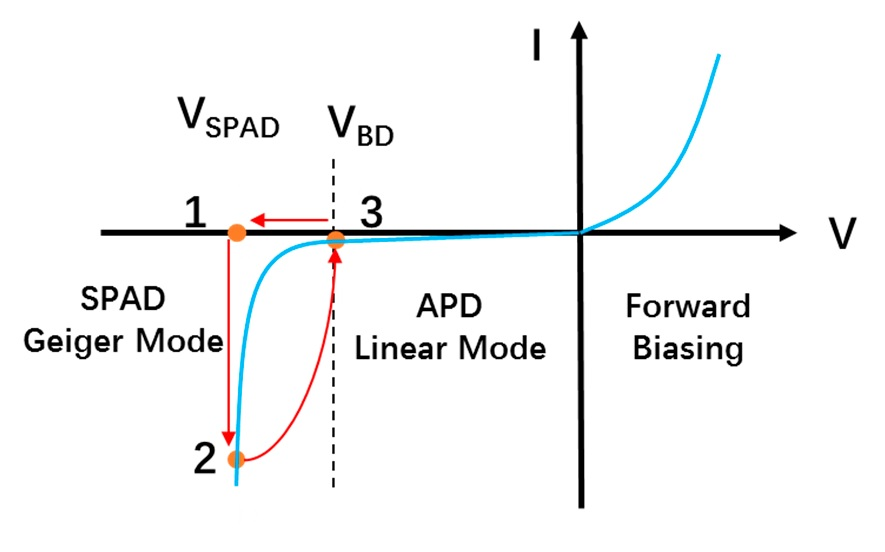
\includegraphics[width=\linewidth]{./ImageFiles/spad_VI.png}
	\end{minipage}
	\caption{Principio di funzionamento di un \textit{single-photon avalanche diode} (SPAD): (a) Processo a valanga in una giunzione p-n polarizzata inversamente; (b) Caratteristica tensione corrente di un diodo SPAD. Immagine tratta da Jiang W. et al. \cite{Jiang2019}.} 
	\label{fig:spad_VI}
\end{figure}

Dal momento che il guadagno di un diodo fotorivelatore a singolo fotone è teoricamente infinito, ha un funzionamento simile a un dispositivo digitale, contando i fotoni incidenti, a differenza dei APDs che in uscita producono una corrente amplificata in funzione dei fotoni incidenti \cite{Jiang2019}. Come anche i PMT, il rumore associato ai diodi SPAD è caratterizzato dal numero di conteggi di buio (DCR), definito come il numero di eventi a valanga in un secondo generati in condizioni di buio. Questi eventi stocastici, possono essere causati da differenti meccanismi. A temperatura ambiente, il fattore che influenza di più il DCR è il meccanismo di generazione-ricombinazione dovuto a portatori liberi generati per agitazione termica. Per cui, questo parametro aumenta all'aumentare della temperatura operativa del diodo. Inoltre, il numero di conteggi aumenta anche all'aumentare della sovratensione $V_{EX}$ applicata \cite{DiFranco2002}, aumentando la probabilità di innescare una valanga e il volume della zona svuotata. Inoltre, un contributo significativo al DCR può essere dato dall'effetto di \textit{afterpulsing} \cite{DiFranco2002}, il quale è causato da portatori provenienti dal precedente evento a valanga, che vengono intrappolati, da difetti presenti nel reticolo del substrato, e rilasciati dopo un certo intervallo di tempo. Se esso è superiore al tempo di \textit{hold off}, essi possono produrre a loro volta un valanga, generando afterpulsing. L'afterpulsing dipende quindi dalla quantità totale di carica che partecipa alla valanga, che aumenta all'aumentare della capacità associata alla giunzione p-n \cite{Palubiak2011}.Inoltre, il fenomeno diventa più evidente all'aumentare del tempo di spegnimento della valanga e all'intensità della corrente, proporzionale a sua volta alla sovratensione applicata aumenta. Un altro parametro che definisce le caratteristiche di un diodo SPAD è l'efficienza di fotorivelazione (PDE), che dipende dal parametro geometrico del \textit{fill-factor} (FF), la probabilità di assorbimento (che dipende dalla lunghezza d'onda) e della probabilità di innesco di un evento a valanga.

I diodi SPAD sono tipicamente realizzati in tecnologia \textit{complementary metal-oxide semiconductor}, che permettono di miniaturizzare la struttura del diodo e ridurre i costi di produzione. nella figura \ref{fig:cmos}(a) si mostra la sezione di una tipica giunzione p-n.
\begin{figure}[tbh]
	\centering
	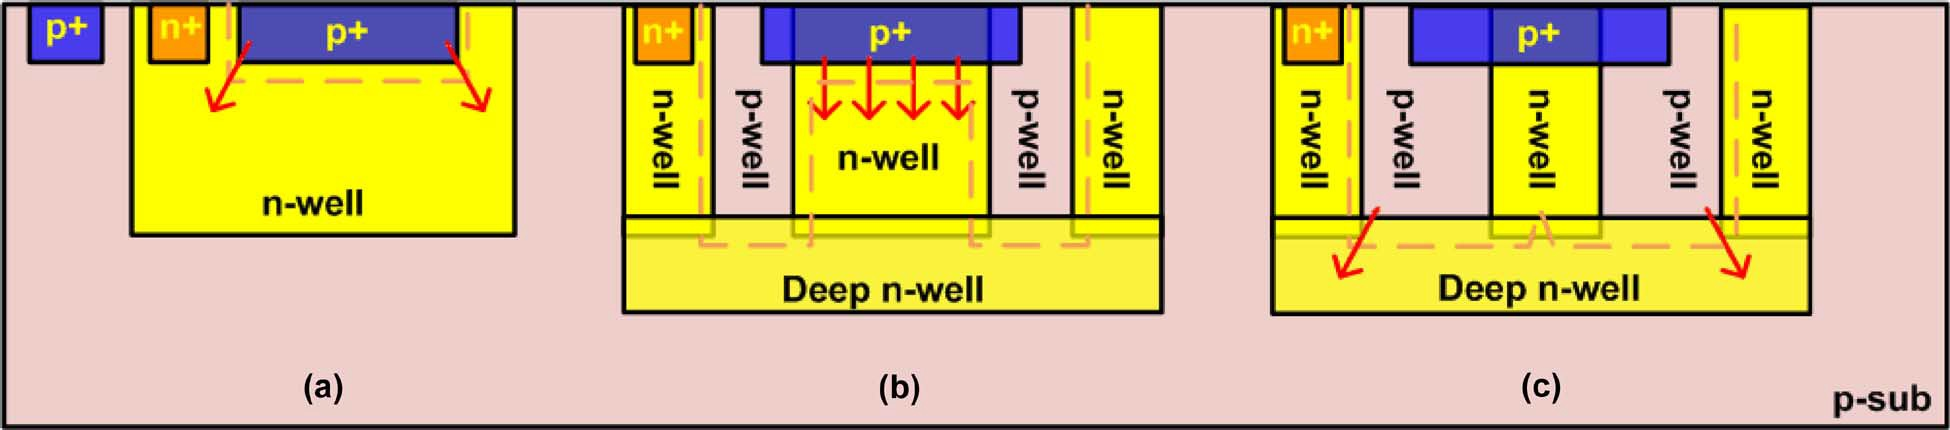
\includegraphics[width=0.8\linewidth]{./ImageFiles/cmos.jpg}
	\caption{Sezione trasversale di possibili realizzazione di un diodo. (a) Tipica giunzione p-n. (b) Tipica struttura di un diodo SPAD e (c) layout di uno SPAD con dimensioni ridotte. Le linee tratteggiate mostrano la regione di svuotamento, mentre le frecce rosse la direzione del campo elettrico. Immagine tratta da Palubiak D. et al. \cite{Palubiak2011}}. 
	\label{fig:cmos}
\end{figure} 
Sebbene questa semplice strutta possa essere utilizzata per realizzare un diodo SPAD, presenta un principale problema: il campo elettrico negli angoli periferici della giunzione (frecce rosse nella figura) raggiunge il valore di breakdown prima dell'area laterale della giunzione \cite{Palubiak2011}. Questo fenomeno è definito come \textit{premature edge breakdown} (PEB). A causa di questo fenomeno non è possibile ottenere un campo elettrico uniforme lungo tutta la regione di svuotamento, influenzando negativamente le performance del diodo. Per questo motivo, sarebbe preferibile utilizzare un andamento circolare della giunzione. Tuttavia, nella tecnologia CMOS non è tipicamente realizzabile. Per eliminare questo fenomeno, è possibile inserire una uno strato drogato p agli angoli della giunzione in modo da aumentare la tensione di breakdown gli angoli (\Fig\ref{fig:cmos}(b)). Lo strato p-well viene isolato dal substrato tramite una regione drogata n (deep n-well layer). Per cui, lo strato p-well aggiunto definisce un anello (denominato \textit{guard ring}) intorno alla regione n-well. Tuttavia, se le regioni p-well si avvicinano troppo, il diodo si comporta di nuovo come una classica giunzione p-n (\Fig\ref{fig:cmos}(c)). Un esempio di soluzione al problema è presentato in Palubiak D. et al. \cite{Palubiak2011}. Nella figura \ref{fig:cmos_2} è rappresentato il dispositivo SPAD realizzato con tecnologia a \SI{130}{\nano\meter}. In questo sensore, la regione n-well che costituisce il guard-ring (\Fig\ref{fig:cmos_2}(a)), non viene estesa fino a toccare lo strato di deep n-well. Questa modifica permette di passare dal classico SPAD (\Fig\ref{fig:cmos}(b)) che utilizza una diodo p+/n-well a un diodo n+/p-well, dove la regione di fotorivelazione è costituita da una zona drogata n+, rendendo possibile un ulteriore miniaturizzazione del sensore controllando la PEB.   
\begin{figure}[tbh]
	\centering
	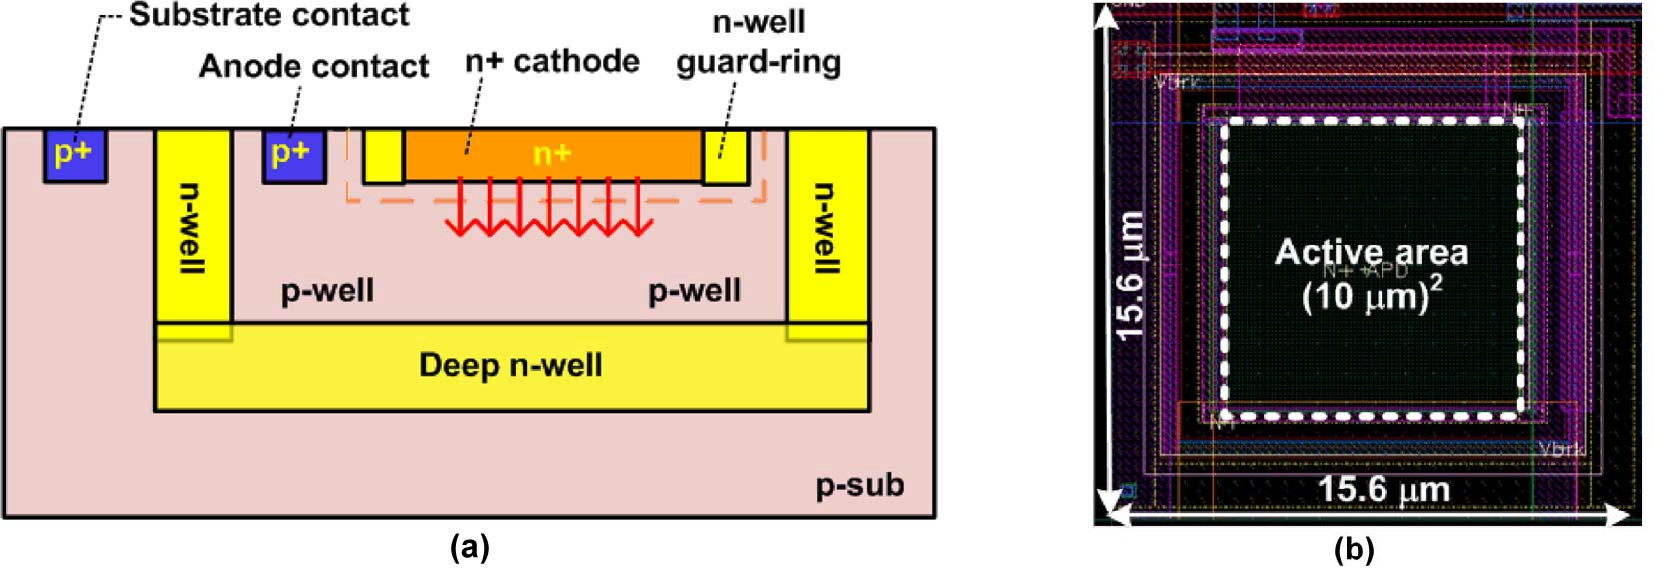
\includegraphics[width=0.8\linewidth]{./ImageFiles/cmos_2.jpg}
	\caption{(a) Vista trasversale del diodo SPAD, che mostra come l'area sensibile è confinata solamente nella zona sottostante la regione drogata n+. (b) Dimensioni del dispositivo SPAD realizzato. Le  Immagine tratta da Palubiak D. et al. \cite{Palubiak2011}}. 
	\label{fig:cmos_2}
\end{figure} 

Una volta che un fotone ha generato l'evento a valanga è possibile vendere un impulso di corrente in uscita al diodo. Per bloccare la valanga, è necessario diminuire la tensione ai capi del diodo al di sotto della tensione di brakdown. L'intervallo tra l'inizio e la fine di un effetto a valanga è chiamato \textit{quenching time}. Il \textit{reset time} si riferisce invece al tempo necessario per riportare il diodo alla tensione di polarizzazione inversa iniziale $V_{BR}+V_{EX}$. I circuiti di quench e reset si dividono in due categorie: PQR (passive quench and reset) e AQR (active quench reset). Un circuito PQR è costituito da una resistenza di valore elevato (\numrange[range-phrase=--]{50}{500}\,\unit{\kilo\ohm}) e già descritto in precedenza. Questi circuiti sono stati largamente utilizzati nella progettazione di pixel SPAD poiché occupano una piccola area, portando a un alto FF e una ridotta capacità parassita. Tuttavia, i PQR hanno alcuni svantaggi. In particolare, a causa del valore elevato della resistenza di queching, porta a una costante di tempo alta associata alla carica della capacità della giunzione, limitando la frequenza operativa di utilizzo del sensore. Per questo motivo sono stati introdotti, i circuiti attivi AQR (\Fig\ref{fig:aqr}).
\begin{figure}[tbh]
	\centering
	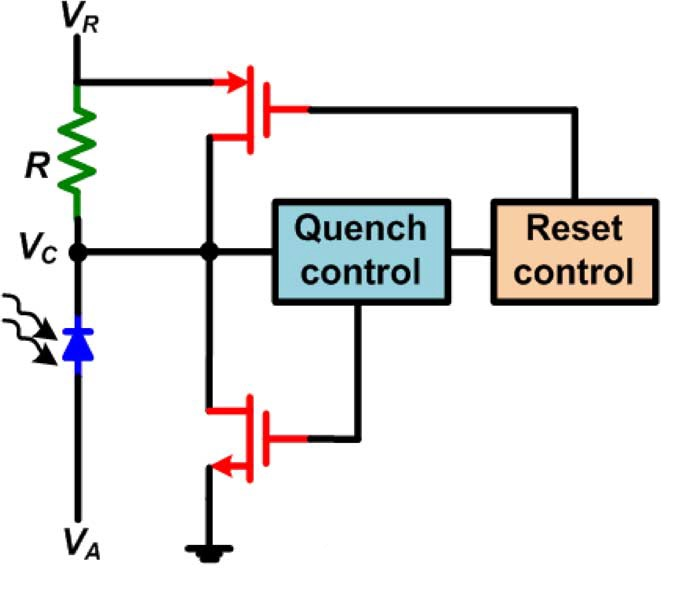
\includegraphics[width=0.6\linewidth]{./ImageFiles/aqr.jpg}
	\caption{Schema semplificato di un circuito \textit{active quench-reset} (AQR). Immagine tratta da Palubiak D. et al. \cite{Palubiak2011}}. 
	\label{fig:aqr}
\end{figure} 
Quando è si sviluppa una valanga, inizia una fase di quenching passivo, come nei circuiti PQR. Dopo un certo intervallo di tempo che dipende da una determinata tensione di soglia (definita dai componenti presenti nel circuito), il \textit{quench control} attiva un transistor nMOS che scarica il diodo a una velocità maggiore. Dopo un certo intervallo di tempo, il circuito di \textit{active reset control} accenderà un transistor pMOS, per un breve istante, riportando la tensione di polarizzazione al valore iniziale (\Fig\ref{fig:aqr_2}).
\begin{figure}[tbh]
	\centering
	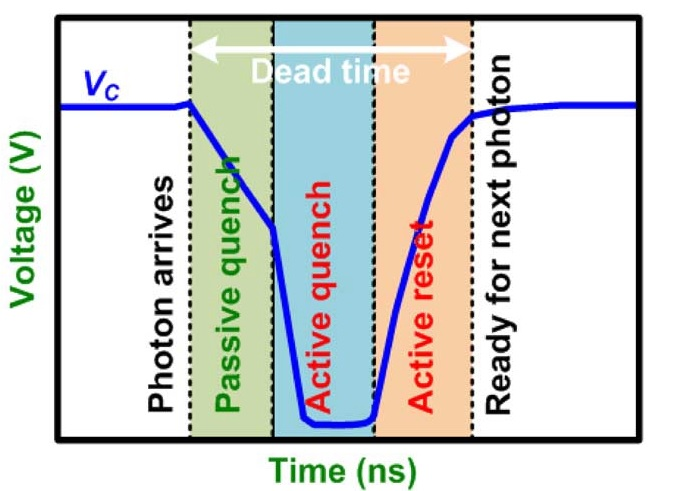
\includegraphics[width=0.6\linewidth]{./ImageFiles/aqr_2.jpg}
	\caption{Andamento nel tempo della tensione V\sub{C} ai capi del diodo. Immagine tratta da Palubiak D. et al. \cite{Palubiak2011}}. 
	\label{fig:aqr_2}
\end{figure} 
I circuiti attivi aumentano la velocità operativa del diodo ma introducono complessità, riducendo il fill-factor e aumentando la capacità parassita associato al circuito.

Affiancando diversi SPAD in modo da formare una matrice e progettando un opportuno circuito di lettura, si definisce un sensore in grado di rilevare fotoni nel piano. Questo tipo di sensore viene definito Analog SiPM. Con il progresso della tecnologia di fabbricazione dei diodi SPAD e grazie alla miniaturizzazione dei componenti nei processi CMOS, sono stati progettati i Digital SiPM, in cui l'elettronica di lettura è direttamente inserita nel sensore. Ciò comporta un miglioramento nelle performance del sensore (riduce il deadtime) e semplifica alcuni circuiti necessari al condizionamento dei segnali utilizzati per gli Analog SiPM.

\clearpage
\subsection{CZT}

\clearpage
\section{Principio di funzionamento}

\clearpage
\section{TOF PET}